\documentclass[a4paper,11pt]{report} % A4, 11 punti, fronte-retro, libro
\usepackage[italian]{babel} % Adatta LaTeX alle convenzioni tipografiche italiane
\usepackage[utf8]{inputenc} % Consente l'uso caratteri accentati italiani
\usepackage{graphicx} % Per le immagini  
\usepackage {fancyhdr} % Per l' ambiente abstract
\pagestyle{fancy}
\renewcommand{\chaptermark}[1]{% 
\markboth{\thechapter.\ #1}{}} 
\renewcommand{\sectionmark}[1]{}
\usepackage{indentfirst} % Indentazione all' inizio dei capitoli
\usepackage{listings}
\usepackage[usenames]{color}
\usepackage{multirow}
\usepackage{multicol} 

\textsc{}\lstnewenvironment{code}[1][]
{\lstset{basicstyle=\small\ttfamily %, columns=fullflexible,
keywordstyle=\bfseries, commentstyle=\color{blue},
language=C,   basicstyle=\small,}}{}
%\lstloadlanguages{C}
\usepackage{url} % Formattazione URLl
\newenvironment{mylisting} % Supporto al codice sorgente
	{\begin{list}{}{\setlength{\leftmargin}{1em}}\item\scriptsize\bfseriesf} %
	{\end{list}}%
\newenvironment{mytinylisting} %
	{\begin{list}{}{\setlength{\leftmargin}{1em}}\item\tiny\bfseries} %
	{\end{list}} %
\newcommand{\fncyblank}{\fancyhf{}} % 
%\newenvironment{abstract} %
\frenchspacing % Non aumentare la spaziatura tra periodi

\begin{document}
%	\frontmatter
		%%%%%%%%%%%%%%%%%%%%%%%%%%%%%%%%%%%%%%%%%%%%%%%%%%%%%%%%%%%
% Fronte

% vspace serve ad aggiungere extra spazio verticale
% em sta ad indicare la grandezza della lettera M maiuscola

% Large indica una dimensione del font di 14.4 pt
% large indica una dimensione del font di 12 pt
% normalsize indica una dimensione del font di 10 pt

% vfill inserisce sufficiente spazio binaco verticalmente per fare in modo che il
% sopra e il sotto del testo siano allieneati col margine superiore e inferiore

\begin{titlepage}
 \begin{center}
     
\includegraphics[width=7cm]{Immagini/unipi.jpg}\\
     \vspace{1em}
     {\Large \textsc{Università degli studi di Pisa}}\\
     \vspace{1em}
     {\Large \textsc{Facoltà di Ingegneria}}\\
     \vspace{2em}
     {\normalsize Corso di laurea in}\\
     \vspace{1em}
     {\Large \textsc{Ingegneria Informatica}}\\
     \vspace{2em}
     {\LARGE \textbf{Realizzazione del supporto }}\\
     \vspace{1em}
     {\LARGE \textbf {per il file system in un nucleo}}\\
     \vspace{1em}
     {\LARGE \textbf {multiprogrammato}}\\
     \vspace{1em}
 \end{center}


\vskip 2cm
  \begin{center}
    \begin{tabular}{c c c c c c c c}
      RELATORI  & & & & & & & CANDIDATO \\
      \large{Prof. Giuseppe Lettieri}   & & & & & & & \large{Giuseppe Pes}\\
      \large{Prof. Enzo Mingozzi} 
    \end{tabular}
  \end{center}

\vskip 1cm
\begin{center}
{\normalsize Anno Accademico 2010/2011}
\end{center}
\end{titlepage}
\clearpage{\pagestyle{empty}\cleardoublepage}
%\clearpage{\pagestyle{empty}\cleardoublepage}

		\tableofcontents
\clearpage{\pagestyle{empty}\cleardoublepage}
\listoffigures
\clearpage{\pagestyle{empty}\cleardoublepage}
%\listoftables
%\clearpage{\pagestyle{empty}\cleardoublepage}

		
	%\mainmatter
		\chapter{Introduzione}
\label{chap:Intro}
\section{Obiettivo}
L'elaborato si propone di descrivere in maniera generale la realizzazione del supporto per il file system in un nucleo multiprogrammato.
\section{Struttura dell'elaborato}
La relazione si compone di 6 capitoli e un'appendice. 
Nel capitolo \ref{cap:FileSystem} si effettua una panoramica generale sul concetto di file system e sulle sue caratteristiche generali.\\
Nel capitolo \ref{cap:Fat}, si descrive con particolare cura il funzionamento del FAT32, mettendo in evidenza le strutture dati di cui è composto e le procedure necessarie per un suo corretto funzionamento. 
Dopo l'introduzione del concetto di file sytem e FAT32, nel capitolo  \ref{cap:Requisiti}, si presentano gli obiettivi del software evidenziando il punto vista dell'utente finale. In questo capitolo analizziamo e sintetizziamo i requisiti utente e software. 
Gli ultimi due capitoli trattano la realizzazione del file system da un punto di vista progettuale. Nel capitolo \ref{cap:Modifiche} si mettono in evidenza tutte le modifiche che sono state introdotte nel nucleo. 
L'ultimo capitolo,infine, individuato dal numero \ref{cap:Struttutra_Progetto}, presenta l'architettura software generale del sistema, mettendo in evidenza i moduli di cui è composto. 

\section{Come Leggere l'elaborato}
Prima di affrontare la lettura di questo elaborato bisogna evidenziare alcuni concetti che verranno usati spesso nell'elaborato. 
\begin{itemize}
  \item Per nucleo si intende il nucleo didattico del Prof. Frosini e Prof. Lettieri, reperibile presso http://calcolatori.iet.unipi.it/. 
  \item Per utente si intende un utilizzatore del nucleo sopracitato. Si assume che l'utente abbia competenze necessarie all'avvio del nucleo e alla scrittura di programmi per questo. 
  \item Il termine sistema si riferisce al sistema file system FAT 32 oggetto della tesi. 
  \item Quando si fa riferimento al file system si intende sempre il FAT 32.  
  \item I termini Partizione e Volume verranno usati come sinonimi. 
\end{itemize}

   
		\chapter{File System}
\label{cap:FileSystem}
In questo capitolo facciamo una introduzione generale al concetto di
file system, mettendo in evidenza gli scopi e le varie
tipologie esistenti.
	\section{Introduzione concetto file System }
        	{\bf Definizione}: 
                \begin{quote}
		\textit{``Un file system è l'insieme dei tipi di dati
           astratti necessari per la memorizzazione, l'organizzazione
           gerarchica, la manipolazione, la navigazione, l'accesso e
           la lettura dei dati.''}
		\end{quote}
         Il file system è la componente del sistema operativo che si
         occupa dell'archiviazione dei dati sui dispositivi di
         memoria secondaria e terziaria, fornendo all'utente finale
         un interfaccia semplice da usare, realizzata mediante il
         concetto di \emph{File}.
         \newline \newline
               {\bf    Definizione}: 
	        \begin{quote}
                \textit{``I File è un insieme di informazioni, correlate e
           registrate in memoria secondaria, cui è stato assegnato un
           nome.''}
         \end{quote}
         Il file system si occupa dell'archiviazione dei file sulla
         memoria secondaria, gestisce le modalità di accesso a questi
         e si occupa anche della protezione dei file associando a essi
         dei privilegi.Tutto questo deve essere fatto in maniera
         trasparente rispetto all'utente finale che non deve avere
         nessuna conoscenza della posizione dei dati nel disco e ne
         come i dischi funzionino.
         \section{Struttura generale}
	 Per poter realizzare tutte queste funzionalità il file
         system è composto da molti livelli distinti. La struttura
         illustrata alla figura \ref{fig:Schema} è un esempio di struttura
         stratificata. Ogni livello si serve delle funzioni del
         livello inferiore per crearne di nuove per il livello
         superiore. 
		\begin{description}
		\item[File system base] Il File system di base è il livello più basso del file
		 system, questo modulo ha lo scopo di colloquiare con il
		 driver del disco inviando dei generici comandi di scrittura e
		 lettura. 
 		\end{description}
        
		\begin{description}
		\item[Il modulo di organizzazione dei file]
		Il  modulo di organizzazione dei file è a conoscenza
		dei file e dei loro blocchi logici, così come dei blocchi
		fisici dei dischi. Conoscendo il tipo di allocazione dei file
		usati e la locazione dei file, può tradurre gli indirizzi
		dei blocchi logici, che il file system di base deve trasferire
		negli indirizzi dei blocchi fisici.
		Il modulo di organizzazione dei file comprende anche il
		gestore dello spazio libero, che registra i blocchi non
		assegnati e li mette a disposizione del modulo di
		organizzazione dei file quando richiesto. 	
		\end{description}

		\begin{description}
		\item[File system logico]
		Il file system logico gestisce i metadati; si tratta
		di tutte le strutture del file system, eccetto gli effettivi
		dati (il contenuto dei file). Il file system logico gestisce
		le struttura  della directory per fornire al modulo di
		organizzazione dei file le informazioni di cui necessità,
		dato un nome simbolico di file. Mantiene le strutture dei
		file tramite i blocchi di controllo dei file (file control
		block,FCB), contenti informazioni sui file, come la
		proprietà,i permessi e la posizione del contenuto. 
                \end{description}
	 Nei file system stratificati la  duplicazione del codice è ridotta al minimo. Il controllo dell'IO e, talvolta, il codice di base del file system, possono 
	  essere comuni a numerosi file system, che poi gestiscono il file system logico e i moduli per l'organizzazione dei file secondo le proprie esigenze. 
          Sfortunatamente, la stratificazione può comportare un maggior overhead del sistema operativo, che può generare un conseguente decadimento delle prestazioni. 
         L'utilizzo della stratificazione e la scelta del numero di strati utilizzati sono aspetti critici nella realizzazione di un file system, in quanto queste scelte 
        incidono sulle prestazioni del sistema.         
	\begin{figure}[h]
 \centering
 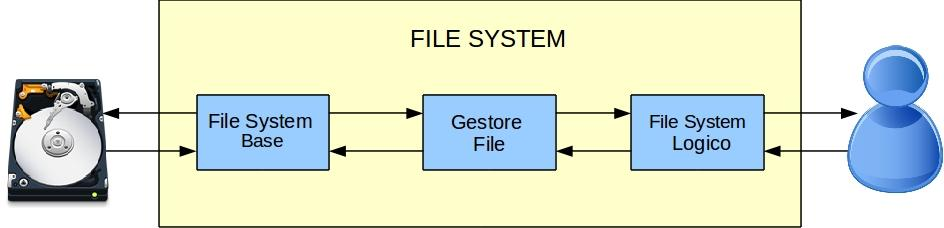
\includegraphics[width=350px,height=100px]{./Immagini/schema.jpg}
 % schema.jpg: 944x228 pixel, 96dpi, 24.98x6.03 cm, bb=0 0 708 171
 \caption{File system stratificato}
 \label{fig:Schema}
\end{figure}

	  \newpage
         \section{Strutture Dati}
         Per realizzare un file system si usano numerose strutture dati, sia nei dischi sia in memoria. Nei dischi, il file system tiene informazioni su come eseguire l'avviamento di un sistema operativo memorizzato nei dischi stessi, il numero totale di blocchi, il numero di locazioni dei blocchi liberi, la struttura delle directory e i singoli file. 
	 In questo paragrafo menzioniamo le più importanti : 
	  \begin{description}
	   \item[Blocco di controllo dell'avviamento] 
	    Il blocco di controllo di controllo dell'avviamento ({\emph boot control block}, contiene le informazioni necessarie al sistema per l'avviamento di un sistema operativo da quel volume; se il disco non contiene un sistema operativo, tale blocco è vuoto. Di solito è il primo blocco di un volume. 
 	  \end{description}
	  \begin{description}
	   \item[Blocchi di controllo dei volumi] 
	Il blocco di controllo dei volumi (\emph volume control block) ciascuno di loro contiene i dettagli riguardanti il relativo volume ( o partizione), come il numero e la dimensione dei blocchi nel disco, il contatore dei blocchi liberi e i relativi puntatori, il contatore dei blocchi di controllo dei file liberi e i relativi puntatori.
 	  \end{description}
	  \begin{description}
	   \item[Strutture delle directory]
	    La Struttura delle directory è la struttura che consente un organizzazione dei file secondo degli schemi logici, unica per ogni volume. 
 	  \end{description}
	  \begin{description}
	   \item[Blocchi di controllo di file]
	    I blocchi di controllo di file {\emph (FCB)}, contiene molti dettagli dei file, compresi i permessi di accesso ai relativi file, i proprietari, le dimensioni e la locazione dei blocchi di dati. 
 	  \end{description}
	  Le informazioni tenute in memoria servono sia per la gestione del file sytem sia per migliorare le prestazioni attraverso l'uso di cache. Questi dati vengono caricati in memoria 
	quando il volume è montato ed eliminati nel momento nel quale viene smontato. 
	    \begin{description}
	     \item[Tabella di montaggio]
	      La tabella di montaggio interna alla memoria che contiene tutte le informazioni attinenti al ciascun volume montato. 
 	    \end{description}
	    \begin{description}
	     \item[Struttura delle Directory]
	      Una parte della struttura delle directory presente nel disco viene carica in memoria in base a quali directory i processi hanno avuto accesso di recente.
 	    \end{description}
	    \begin{description}
	     \item[Tabella generale file aperti]
	      La tabella generale dei file aperti  contiene una coppia del FCB per ciascun file aperto all'interno del sistema operativo.  
 	    \end{description}
	      \begin{description}
	       \item[Tabella locale file aperti] 
		La tabella locale dei file aperti è una struttura dati associata ad ogni processo che contiene tutte le informazioni attinenti hai file aperti da quel determinato processo, tipicamente mantiene dei puntatori ai FCB della tabella globale dei file aperti. 
 	      \end{description}
         \section{Metodi di allocazione} 
         Il problema principale che il file system deve risolvere è l'allocazione dello spazio per i file nel disco. Questo è un problema complesso da cui dipende l'efficienza del file system stesso, perché un file system efficiente deve fornire una gestione dello spazio ottimale riducendo al minimo gli overhead e un accesso rapido al contenuto dei file. 
         Esistono tre metodi principali per l'allocazione dei file, ognuno con i suoi vantaggi e svantaggi,in base alle esigenze che si hanno e il contesto nel quale il file system andrà a lavorare si adotterà il metodo più idoneo.
         
      \begin{description}
       \item[Allocazione contigua]
        La base di questo metodo di allocazione consiste nell'occupare per ogni file un insieme di blocchi contigui del disco. Il principale vantaggio di questo metodo di allocazione è che si rendono trascurabili il numero di posizionamenti  richiesti per accedere al contenuto del file , così come è trascurabile il tempo di ricerca quando quest'ultimo è necessario.
      Il primo problema di cui è affetto questo metodo è l'individuazione dello spazio libero, in quanto il gestore dello spazio libero deve trovare uno spazio libero formato da blocchi contigui che sia in grado di contenere la quantità di dati da immagazzinare, per fare questo si possono usare degli algoritmi per la scelta del buco libero ( esempi sono best-fit las-fit first-fit), ma tutti questi sono affetti dal problema della frammentazione esterna. 
      Il secondo problema che si presenta usando questo metodo è che può risultare impossibile estendere il file dopo il suo allocamento, in quanto lo spazio oltre le due estremità del file può essere già in uso, quindi non è possibile ampliare il file in modo continuo.
      Questa metodologia può essere affiancata da varie estensioni per renderla in grado di affrontare i problemi precedenti. 
      Questo modello di allocazione è molto efficiente come tempi di accesso ai dati, ma le problematiche attinenti alla frammentazione dello spazio lo rendono usabile solo in particolari condizioni, e anche con l'introduzione di varie estensioni questi problemi vengono ridotti ma non eliminati. 
       \end{description}

      \begin{description}
       \item[Allocazione Concatenata]
        Il metodo di allocazione Concatenata risolve tutti i problemi di cui era afflitto il metodo di allocazione contigua.Con questo tipo di allocazione, infatti , ogni file è composto da una lista concatenata di blocchi del disco i quali possono essere sparsi in qualsiasi punto del disco stesso. Per poter risalire a un file nel disco la directory deve contenere 
        un puntatore al primo blocco, e ogni blocco contiene il puntatore al blocco successivo fino all'ultimo blocco della lista, che conterrà un puntatore  speciale che indicherà che questo è l'ultimo blocco. Quindi per eseguire la lettura si legge l'indirizzo del primo blocco  dalla directory fino a raggiungere la posizione ricercata mediante la lista di blocchi.
        Il primo problema di questo metodo è che i file possono essere usati in modo efficiente solo con accessi sequenziali, mentre l'accesso diretto al file estremamente inefficiente in quanto bisogna scorrere tutta la lista di blocchi prima di arrivare alla posizione ricercata. 
        Un altro svantaggio è lo spazio richiesto per il salvataggio dei puntatori dei vari blocchi. La soluzione più comune a questo problema consiste nel riunire un certo numero di blocchi contigui in {\bf cluster}, e nell'allocare cluster invece di blocchi. Questa soluzione però incrementa la frammentazione interna che era minore con l'allocazione di blocchi.
        Il secondo problema riguarda l'affidabilità. Essendo i file gestiti mediante liste se si corrompe un puntatore si ha la perdita del file in quanto non è più possibile seguire la lista. Esistono varie soluzioni a questo problema, la prima consiste nell'usare liste doppiamente concatenate, oppure usare una gestione ridondante dei puntatori. 
        Un'importante versione del metodo di allocazione Concatenata e quello {\bf FAT} che verrà analizzato in dettaglio nel paragrafo §\ref{cap:Fat}, questo risolve in modo efficiente il problema dell'accesso in modo diretto. 
       \end{description}
      \begin{description}
        \item[Allocazione indicizzata]
        Il metodo di allocazione indicizzata risolve il problema, raggruppando i puntatori in una sola locazione che prende il nome di {\bf blocco indice}. Ogni file ha il proprio blocco indice, si tratta di un array  d'indirizzi di blocchi del disco. L'\textit{i}-esimo elemento del blocco indice punta all'\textit{i}-esimo blocco del file. Per poter risalire al file,la directory contiene il puntatore al blocco indice del file. Con questa soluzione sono efficienti sia gli accessi sequenziali,  che gli accessi diretti e in più non si ha frammentazione esterna.
        Anche questo metodo di allocazione è afflitto da una problematica, che consiste nello scegliere la grandezza del blocco indice, infatti se si sceglie una grandezza troppo piccola non si possono allocare file di grandi dimensioni, invece se si sceglie una grandezza del blocco indice troppo elevata si introduce uno spreco di spazio perché la maggior parte dei puntatori interni del blocco indice rimangono inutilizzati. 
        Per gestire questa situazione si usano vari approcci : 
        \begin{itemize}
         \item \textbf{Schema concatenato} Un blocco indice è formato da un solo blocco del disco, e per realizzare più blocchi vengono concatenati più blocchi indice tra loro.
        \end{itemize}
        \begin{itemize}
         \item \textbf{Indice a più livelli} Un blocco indice di primo livello punta ai blocchi indice di secondo livello che, a loro volta, puntano ai blocchi dei file, così si crea una struttura ad albero che permette l'allocazione di grandi file.
        \end{itemize}
        \begin{itemize}
         \item \textbf{Schema combinato} Consiste nell'utilizzare entrambe le soluzioni precedenti, associando ad ogni file dei puntatori diretti ai blocchi dei file , e dei puntatori a blocchi indice di vario livello in base alle esigenze. In questo modo con gli indirizzamenti diretti si possono gestire i file di piccole dimensioni senza introdurre rilevanti perdite di spazio, e quando lo spazio indirizzato da questi risulta insufficiente, si utilizzano i blocchi indice a più livelli. 
        \end{itemize}
        \end{description}
         Come esposto esistono una varietà di metodi di allocazione dei dati sul disco, ognuno di questi ha i suoi vantaggi e svantaggi. Il metodo di allocazione da adottare in un file system  è legato al  contesto in cui andrà a lavorare quel file system, soprattutto con quale tipologia di file, così facendo  si cerca di ottimizzare al meglio le prestazioni.
         Spesso però questo non è sufficiente, e per ottenere dei file system efficienti, bisogna inserire delle estensioni per migliorarne le prestazioni, alle volte a discapito della generalità del file system steso.
         \section{Metodi di gestione dello spazio libero} 
         Un altro aspetto importante del file system  è la gestione dello spazio libero. Il sistema deve conservare una lista dello spazio libero dove sono registrate tutte le locazioni libere del disco. Per creare un file occorre cercare nella lista dello spazio libero la quantità di spazio necessaria e assegnarla al nuovo file, quindi rimuovere questo spazio dalla lista. Quando si cancella un file, si aggiungono alla lista dello spazio libero i blocchi del disco ad esso assegnati. 
         La lista dello spazio libero può essere implementata in vari modi: 
         \begin{itemize}
          \item \textbf{Mappa di BIT} Con questo metodo si realizza la lista mediante \textit{una mappa di bit}.Ogni blocco è rappresentato da un bit: se il blocco è libero, il bit è 1, se il bit è assegnato il bit è 0. Il vantaggio principale è che il metodo è molto semplice da realizzare ed efficiente.
         \end{itemize}
          \begin{itemize}
           \item \textbf{Lista concatenata} Con questo metodo si collegano tutti i blocchi liberi, e si tiene un puntatore al primo blocco libero in una particolare posizione del disco. Quando si ha necessità di un blocco si preleva  semplicemente il primo della lista.Questo metodo non è efficiente se si ha necessità di scorrere la lista dei blocchi.    
          \end{itemize}
          \begin{itemize}
           \item\textbf{ Conteggio} Questo metodo, sfrutta l'idea che più blocchi liberi siano contigui tra di loro, in questo modo si può tenere traccia dell'indirizzo del primo blocco ed il numero di blocchi liberi contigui che seguono il primo blocco, e anche se la coppia indirizzo più contatore occupano più di un indirizzo normale, la lista finale comunque ha una lunghezza inferiore.
          \end{itemize}
            Come nel caso  della scelta del metodo di allocazione anche qui bisogna scegliere l'implementazione in base al contesto in cui ci andrà a lavorare.
         \section{Conclusioni}
            Come si è visto in questa sezione il file system è un oggetto complesso di fondamentale importanza per il sistema operativo.  Il processo di realizzazione di un file system è molto lungo è complesso, e deve essere curato nei minimi particolari per cercare di ridurre al minimo gli errori, si pensi alle conseguenze che avrebbero degli errori di programmazione su una parte così delicata del sistema, si potrebbero avere  perdite di dati, accessi non autorizzati ai file e così via.
            Nella scelta del file system da implementare abbiamo scelto il FAT per la sua semplicità implementativa tralasciando le prestazioni in quanto il contesto in cui lavorerà è un semplice sistema didattico. 

\clearpage{\pagestyle{empty}\cleardoublepage}

%%% Local Variables: 
%%% mode: latex
%%% TeX-master: "tesi"
%%% End: 

		\chapter{FAT 32}
\label{cap:Fat}
    Nel presente capitlo introduciamo alcuni concetti generali riguardanti il file system FAT. 
    Successivamente procederemo con un maggior dettaglio analizzando le varie strutture di cui è composto e le procedure mediante le quali i dati vengono salvati e prelevati dal disco. 
  \section{Carateritiche}
  \label{sec:Carateristiche}
    La File Allocation Table, in sigla FAT, è un file system sviluppato inizialmente da Bill Gates e Marc McDonald. È il file system primario per diversi sistemi operativi DOS e Microsoft Windows fino alla versione Windows ME.\\
    La FAT è relativamente semplice ed è supportata da moltissimi sistemi operativi. Queste caratteristiche la rendono adatta ad esempio per i Floppy Disk e le Memory Card e può anche essere utilizzata per condividere dati tra due sistemi operativi diversi.\\
    Il più grande problema del File System FAT è la \textbf{frammentazione}. Quando i file vengono eliminati, creati o spostati, le loro varie parti si disperdono sull'unità, rallentandone progressivamente la lettura e la scrittura. Una soluzione a questo inconveniente è la deframmentazione, un processo che riordina i file sull'unità. Questa può durare anche diverse ore e deve essere eseguita regolarmente per mantenere le prestazioni dell'unità.\\
    Esistono varie versioni di questo file system, in questa sede analizziamo soltanto il FAT32. \\ 
    Il FAT32 presenta alcuni limiti, si possono gestire volumi che hanno una grandezza compresa tra i 512MB e 32 GB, questi limiti sono imposti dalle routine Microsoft, infatti esistono routine di terze parti che permettono di superare questi limiti. \\
    Il file system FAT possiede anche un limite sulla grandezza massima dei file che non può eccedere i 4GB. \\

   \section{Struttura}
       Il File system FAT usa un criterio di allocazione dei dati basato sull'utilizzo di liste concatenate. Per poter rintracciare queste liste, vengono salvate nella FAT presente sul disco. 
	Grazie all'utilizzo della tabella FAT viene anche risolto il problema della gestione dello spazio libero. Il funzionamento della FAT è ampiamente spiegato nel paragrafo \ref{GestioneFat}.\\
      La struttura generale di un volume FAT32 è composta da tre regioni principali: 
        \begin{enumerate}
           \item  \textbf{Regione riservata} Regione nella quale troviamo tutte le informazioni di basso livello attinenti al volume
           \item  \textbf{Regione FAT}  Regione nella quale è presente la tabella FAT indispensabile per la gestione dei dati sul disco. 
           \item  \textbf{Regione Data} Regione nella quale sono presenti i dati veri e propri.
         \end{enumerate}
    
    \begin{figure}[h]
    \centering
    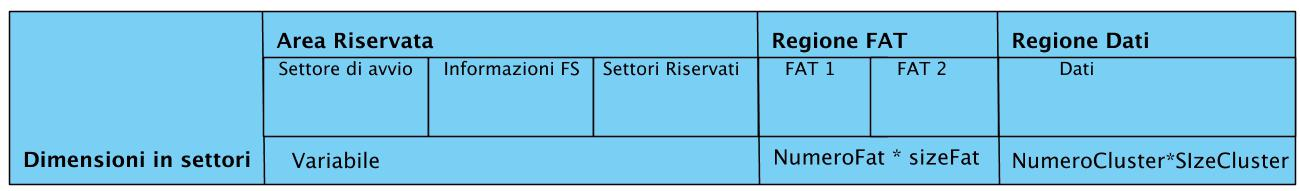
\includegraphics[width=350px,height=70px]{./Immagini/struttura.jpg}
     % struttura.jpg: 1300x191 pixel, 96dpi, 34.40x5.05 cm, bb=0 0 975 143
    \caption{Struttura Volume FAT}
    \label{Fig.: Struttura Volume FAT32}
    \end{figure}

    \subsection{Regione Riservata}

            La regione riservata è la prima regione che troviamo nel volume e contiene tutte le informazioni di basso livello necessarie per un corretto funzionamento del file system stesso. A sua volta questa regione è suddivisa in zone diverse. 
            \begin{itemize}
             \item \textbf{Boot Sector} Questa è la prima struttura presente in un volume FAT, occupa il primo settore del volume  (settore zero) ed è la più importante della regione riservata.\\
	      Il Boot sector include un'area chiamata \textbf{BIOS Parameter Block (BPB)} che contiene alcune informazioni base per il funzionamento del file system quali ad esempio tipo del file system e posizione delle altre regioni nel disco. Il BPB occupa i byte dall'offset 0x1B fino all'offset 0x34 del Boot Sector. \\
	      Oltre al BPB nel boot sector troviamo anche il codice del boot loader necessario per avviare un sistema operativo.
	     La successiva tabella rappresenta schematicamente la struttura del boot sector di un volume FAT32 :
	  
		      \begin{center}
		      \begin{tabular}{|r|r|l|}\hline
			  \textbf {Offset} & \textbf{Lunghezza} & \textbf{Descrizione}\\\hline
			  0x00 & 3 & Salta istruzione\\\hline
			  0x03 & 8 & Nome	\\\hline
			  0x0B & 2 & Estensione\\\hline
			  0x0D & 1 & Bytes per settore \\\hline
			  0x0E & 2 & Numero dei settori di riserva\\\hline
			  0x10 & 1 & Numero di tabelle FAT \\\hline
			  0x11 & 2 & FAT32 vale 0 \\\hline
			  0x13 & 2 & Settori totali. \\\hline
			  0x15 & 1 & Tipo di descrittore. \\\hline
			  0x16 & 2 & Settori per FAT (per FAT12/16) \\\hline
			  0x18 & 2 & Settori per traccia \\\hline
			  0x1A & 2 & Numero di testine \\\hline
			  0x1C & 4 & Settori nascosti \\\hline
			  0x20 & 4 & Totale settori. \\\hline
			  0x24 & 4 & Settori occupati da una FAT \\\hline
			  0x28 & 2 & FAT flags \\\hline
			  0x2A & 2 & Versione \\\hline
			  0x2C & 4 & Cluster Root Directory \\\hline
			  0x30 & 2 & Numero settore FS Information \\\hline
			  0x32 & 2 & Numero settore di Backup \\\hline
			  0x34 & 12 & Riservato \\\hline
			  0x40 & 1 & Numero Driver \\\hline
			  0x41 & 1 & Riservato \\\hline
			  0x42 & 1 & Firma estesa \\\hline
			  0x43 & 4 & ID \\\hline
			  0x47 & 11 & Volume Label \\\hline
			  0x52 & 8 & FAT File sytem type\\\hline
			  0x5A & 420 & Codice Boot loader\\\hline
			  0x1FE & 2 & Firma boot sector\\\hline
		      \end{tabular}
		      \end{center}



	     \end{itemize}
     
	  

	     \begin{itemize}
	     \item \textbf{Fat Information Sector}
	  
	      Introdotto con la FAT32 per accelerare i tempi di accesso di alcune operazioni (i.e. la quantità di spazio libero), occupa generalmente il settore 1, nel record di avvio 0x30. Ha dimensione pari a 512 byte. Contiene un campo nel quale è specificato lo spazio libero rimanente ( offset 0x1E8 ) e il primo cluster dal quale iniziare la ricerca del cluster libero (oofset 0x1F0).
	      \newpage
	      La tabella successiva riepiloga i vari campi :
		      \begin{center}
		      \begin{tabular}{|r|r|l|}\hline
			  \textbf {Offset} & \textbf{Lunghezza} & \textbf{Descrizione}\\\hline
			  0x00  & 4  & Firma File System Info\\\hline
			  0x04  & 480&Riservati	\\\hline
			  0x1E4 & 4  & Firma File System Info\\\hline
			  0x1E8 & 4  & Numero cluster liberi \\\hline
			  0x1EC & 4  &  Cluster dal quale iniziare la ricerca \\\hline
			  0x1F0 & 14 &  Riservato \\\hline
			  0x1FE & 2  &  Firma File System Info \\\hline
		      \end{tabular}
		      \end{center}
 	    \end{itemize}
	  

	    \begin{itemize}
	       \item \textbf{Settori Riservati}
	      Alcuni settori riservati, sono a disposizione per essere usati per rimpiazzare i settori che sono danneggiati nel disco. 
	    \end{itemize}

    \subsection{Regione Fat}
	\label{sec:RegioneFat}
	      La regione FAT è la regione del disco nella quale sono salvate la tabelle FAT. Per avere una maggior sicurezza nel salvataggio dei dati sono presenti per default due tabelle FAT. Il numero di tabelle 
	      presenti nel disco e contenuto nel boot sector ed è configurabile in fase di formattazione.
    \subsection{Regione Dati}
	      La regione Dati è la regione che inizia successivamente alla regione FAT ed è quella nelle quali sono presenti i veri propri dati. 
	      Questa regione è vista dal file system come suddivisa in un certo numero di blocchi di grandezza uguale. Anche in questo caso tutte le informazioni necessarie per la gestione dei blocchi e più in generale della zona dati sono presenti nel Boot sector.
    \section{Getione Fat}
    \label{GestioneFat}
        Dopo aver presentato la struttura generale di un volume FAT 32, analizziamo il meccanismo con il quale vengono salvati i dati. 
	Una partizione è suddivisa in \textbf{cluster} di egual grandezza. I cluster sono dei blocchi di spazio continuo, la cui grandezza dipende dal tipo di file system e dalla grandezza della partizione. 
       Tipicamente la grandezza di un cluster oscilla tra i 2kB e 32 kb ed è stabilita in fase di formattazione.\\
        Ogni file può occupare uno o più cluster in base alla sua grandezza, quindi il file viene rappresentato da una catena di cluster. Le catene sono realizzate mediante una lista concatenata semplice.
        L'insieme dei cluster di cui è composto un file non necessariamente vengono salvati in posizioni adiacenti, ciò comporta una dispersione dei cluster per tutto il disco con un degrado delle prestazioni. 
	Questo fenomeno prende il nome di \textbf{frammentazione}.\\
	La tabella Fat è composta da entry a 32 bit ed posizionata nella regione FAT ( vedi § \ref{sec:RegioneFat} ). Lo scopo di tale tabella è quello di mappare tutti i cluster di cui è composto un volume con la relativa entry. 
	Ogni entry può assumere i seguenti valori : 

	  \begin{itemize}
	   \item Il numero del cluster successivo.
	  \end{itemize}

	  \begin{itemize}
	   \item Il valore speciale di fine catena (EOC)
	  \end{itemize}

	  \begin{itemize}
	   \item Il valore speciale che segnala il cluster come riservato
	  \end{itemize}

	   \begin{itemize}
	    \item  Il valore speciale che segnala il cluster come mal funzionante
	  \end{itemize}

	  \begin{itemize}
	   \item Zero che identifica il cluster come libero
	  \end{itemize}
    
    Usando questa tecnica si crea una corrispondenza univoca tra i cluster del disco e le entry della tabella Fat. Per esempio, se si volesse sapere lo stato del cluster 42 è sufficiente analizzare l'entry numero 42 della tabella. \\
    La struttura della FAT è molto semplice, e di conseguenza anche le operazioni per la gestione dei file risultano essere semplificate.\\
    Infatti per ricercare un cluster libero si scorre la tabella finché non si trova un cluster marcato come libero.
    Per rintracciare tutti i cluster di cui è formato un file è sufficiente conoscere il primo cluster della catena.
    Utilizzando il numero del primo cluter come indice nella tabella si può risalire al cluster successivo, se presente, poiché il suo valore è contenuto nell'entry letta. Usando il valore presente nella nuova entry si può proseguire nella ricerca dei cluster usando la stessa procedura.\\
    La ricerca terminerà quando nell'entry della tabella è presente il valore EOC.
    Le  prime due entry nella FAT contengono speciali valori. La prima entry contiene una copia del media Descriptor ( Descrive il device, contenuto nel boot sector, offset 0x15). I rimanenti bit vengono settati ad 1.\\ 
    La seconda entry contiene il valore di \textit{End Of Chain}, cioè il valore usato per indicare la terminazione di una catena di cluster. I due Bit più significativi di questa entry sono usati per identificare lo stato di occupato del disco e rilevare possibile errori di montaggio.\\ 
    Poiché le prime due entry sono riservate il primo cluster utile della tabella FAT, risulta essere il 2. Il cluster 2 tipicamente è il primo cluster della catena che rappresenta la root directory. \\
    La tabella successiva riassume i valori che possono assumere le entry FAT e il loro significato.\\

    \begin{center}
\begin{tabular}{|c|c|}\hline
\textbf {FAT32} & \textbf{Descrizione}\\\hline
0x00000000 & Cluster Libero\\\hline
0x00000001 & Riservato\\\hline
0x00000002-0x0FFFFFEF & Cluster usabili\\\hline
0x0FFFFFF0-0x0FFFFFF6 & Riservati\\\hline
0xFFFFFF7 & Bad Cluster\\\hline
0x0FFFFFF8-0xFFFFFFFF & End Of Chain\\\hline
    \end{tabular}
    \end{center}

Come si può notare dai Valori della tabella il FAT32 utilizza solamente 28 bit per indicizzare le varie entry della tabella FAT, solitamente i 4 bit più significativi sono settati a zero, ma essendo riservati il loro valore non deve essere modificato. 

    \section{Gestione Directory}
    \label{gest:dir}
Una \textbf{tabella directory} è un file speciale che che rappresenta una cartella.
Ogni riga di questa tabella prende il nome di \textbf{entry} e viene associato ad un file.  Un \textbf{entry} è una struttura dati formata da 32 byte, che contiene le informazioni necessarie per la gestione dei file. 
Sono state introdotte nel FAT32 due tipi di entry diverse. \\
Il primo tipo, presente sin dalla prima versioni del FAT 32 ha lo scopo di contenere le informazioni necessarie per la gestione dei file. La tabella successiva rappresenta tale entry : 

\begin{center}
\begin{tabular}{|l|c|l|}\hline
\textbf{Offset} & \textbf{Lunghezza} & \textbf{Descrizione}\\\hline
0x00 & 8 & Nome file\\\hline
0x08 & 3 & Estensione File\\\hline
0x0B & 1 & Attributi\\\hline
0x0C & 1 & Riservato\\\hline
0x0D & 1 & Tempo creazione ms\\\hline
0x0E & 2 & Tempo creazione\\\hline
0x10 & 2 & Data di creazione\\\hline
0x12 & 2 & Data Ultimo accesso\\\hline
0x14 & 2 & 2 byte piu significativi indirizzo cluster\\\hline
0x16 & 2 & Tempo Ultimo Modifica\\\hline
0x18 & 2 & Data ultimo modifica\\\hline
0x1A & 2 & 2 byte meno significativi cluster\\\hline
0x1C & 4 & Grandezza file\\\hline
\end{tabular}
\end{center}

I campi principali sono il nome, formato da 8 caratteri più 3 caratteri di estensione, entrambi codificati secondo il set di caratteri OEM. 
L'insieme di questi due campi d'ora in poi verrà riferito con il termine nome corto. \\
Il nome corto del file viene generato mediante un algoritmo fornito dalla Microsoft stessa, il quale si occupa di risolvere le problematiche che nascono nel caso in cui siano presenti nomi simili\footnote{Per il concetto di Nomi simili si intendono nomi uguali per i primi 8 caratteri.}, nella stessa cartella.\\
Le altre due informazioni principali presenti in questa struttura sono il numero del primo cluster, necessario per risalire alla catena di cui è composto un file e la grandezza del file, necessaria per 
eseguire le operazioni di scrittura e lettura in maniera corretta. 
Sin dalla prima versione, la lunghezza del nome del file a soli 11 caratteri è stato un limite.\\
Per superare questo limite si è deciso di introdurre delle entry il cui unico scopo era quello di estendere il nome dei file. Questo tipo di entry è riassunta nella successiva tabella.   

\begin{center}
\begin{tabular}{|l|c|l|}\hline
\textbf{Offset} & \textbf{Lunghezza} & \textbf{Descrizione}\\\hline
0x00 & 1  & Indice\\\hline
0x01 & 10 & Nome1\\\hline
0x0B & 1  & Attributi\\\hline
0x0C & 1  & Tipo\\\hline
0x0D & 1  & Checksum\\\hline
0x0E & 12 & Nome2\\\hline
0x1B & 2  & Riservato\\\hline
0x1D & 4  & Nome3\\\hline
\end{tabular}
\end{center}

Queste entry occupano le posizioni che precedono la entry con le informazioni per la gestione dei file. Il nome inserito in questo tipo di entry d'ora in avanti verrà identificato con il termine nome lungo.
Per essere sicuri di associare il nome lungo alla giusta entry, è presente il campo checksum che costituisce il risultato della funzione checksum fornita dalla Microsoft calcolata sul nome corto. 
Per poter risalire a tutte le entry che formano il nome lungo è sufficiente seguire l'indice presente nella prima posizione, finché non si raggiunge l'ultima entry identificata da un marcatore di fine lista.
Con questa soluzione i nomi gestibili da un file system FAT32 possono raggiungere la lunghezza di 255 caratteri. 

\begin{figure}[h]
 \centering
 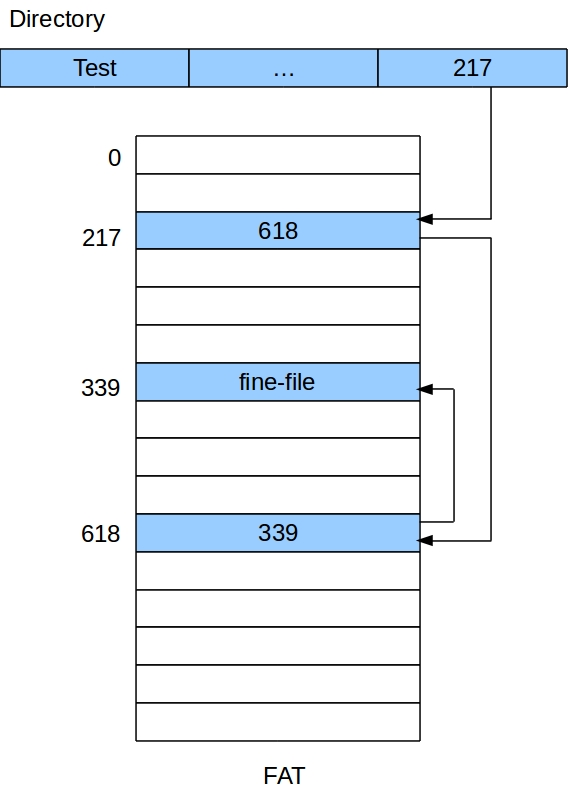
\includegraphics[width=250px,height=300px]{./Immagini/fat.jpg}
 % fat.jpg: 568x806 pixel, 72dpi, 20.04x28.43 cm, bb=0 0 568 806
 \caption{Esempio di una catena FAT}
 \label{Fig.:FAT}
\end{figure}


    \section{Differenze Specifiche}
     Non tutte le specifiche Microsoft esposte nei paragrafi precedenti sono state rispettate, o per aumentare l'efficienza del sistema generale o per avere delle semplificazioni realizzative. 
     La differenze con le specifiche Microsoft sono: 
    
     \begin{itemize}
    
     \item Le tabelle fat di backup vengono ignorate. Ho scelto di ignorare le tabelle di backup per una questione di efficienza, altrimenti ogni scrittura sulla  FAT primaria comporterebbe anche delle scritture 
     nelle FAT di backup che comprometterebbero le prestazioni. Per migliorare quest'aspetto si potrebbe inserire un meccanismo che ad intervalli regolari copia la FAT  primaria nelle FAT di backup.\\
 
     \item Il parametri presenti nel settore Fat Information Sector  la gestione delle zone libere del disco sono stati ignorati in quanto per semplificare e ottenere delle prestazioni migliori si è scelto di caricare l'intera FAT in memoria, quindi la ricerca di un cluster non comporta nessuna operazione sul disco.\\

     \item Ho ignorato i settori di backup del boot sector e in generale la gestione dei settori danneggiati per semplificare la gestione della FAT.\\

     \item Ho ignorato il problema della frammentazione. \\

       
     \end{itemize}
    \section{Conclusione}
    In questo capitolo è stata fatta un introduzione molto semplice al funzionamento del FAT, per eventuali approfondimenti fare riferimento alla documentazione microsoft. 
     Come si è potuto notare dalle spiegazioni dei capitoli precedenti il file system risulta essere molto facile da un punto di vista implementativo. 
      Se si analizzano le prestazioni e i limiti di questo file system      si nota che è poco scalabile e le prestazioni con grandi quantità di dati sono molto scarse, rendendolo quasi inutilizzabile. 
     Un modo per migliorare le prestazioni del file system è l'introduzione di un sistema di cache delle scritture / letture. Questa soluzione è quella adottata nella maggior parte dei sistemi operativi commerciali, 
     che grazie altra struttura modulare ( spiegata nel capitolo § \ref{cap:Struttutra_Progetto} ) posso essere introdotti anche qui. 
      
\clearpage{\pagestyle{empty}\cleardoublepage}

%%% Local Variables: 
%%% mode: latex
%%% TeX-master: "tesi"
%%% End: 
		\chapter{Analisi e specifica dei requisiti}
\label{cap:Requisiti}
Nel presente capitolo si presenta il contesto nel quale il sistema andrà a lavorare, 
si analizzeranno le principali esigenze di un utente e, in termini generali, si mostrerà come il sistema risponde ed interagisce con l'utente. 

\section{Analisi Dominio}
Il  sistema  oggetto della tesi è un file system sviluppato per il nucleo didattico del Prof. Frosini e Prof. Lettieri, che verrà inserito nella versione SVN 568.\\
Il nucleo è diviso in tre moduli distinti, sia logicamente che in fase di linking, come di seguito sinteticamente mostrato : 
\begin{description}
 \item[Modulo Sistema]
  è il modulo principale del nucleo. In questo modulo vengono inizializzate le principali funzionalità di un kernel di cui sono importanti esempi la memoria virtuale e i processi.
  Questo modulo è in esecuzione con i privilegi di sistema. 
 \end{description}
 \begin{description}
  \item[Modulo IO]
  è il modulo nel quale vengono gestite le periferiche di input ed output. Anche questo modulo ha necessità dei privilegi Sistema per operare correttamente. 
  \end{description}
  \begin{description}
   \item[Modulo Utente]
  il modulo che gestisce i programmi utente. Questo modulo va in esecuzione con i privilegi utente. 
   \end{description}
Il file system per poter lavorare correttamente deve usare particolari istruzioni e/o strutture dati accessibili solamente dal livello sistema; si è perciò valutato opportuno inserire il file system nel modulo IO.\\ 
Tale scelta soddisfa anche la necessità di poter sfruttare tutte le potenzialità della memoria virtuale, necessaria per maneggiare le grandi strutture dati di cui è composto.

\section{Requisiti utente}
      In questa sezione analizziamo i requisti utente, cioè quello che l'utente si aspetta dal sistema. 
      L'applicazione deve fornire all'utente finale un file system funzionante compatibile con le specifiche del FAT32. Il file system deve mettere a disposizione delle funzionalità per la gestione dei file e delle cartelle da parte dell'utente.\\
      Più precisamente le specifiche dei requisiti per la gestione dei file sono : 
	\begin{enumerate}
	 \item L'utente deve poter creare ed eliminare i file;
	 \item L'utente deve poter scrivere e leggere  su un file;
	 \item L'utente deve poter stabilire la posizione all'interno del file dove effettuare le varie operazioni.
	\end{enumerate}
	
	Le specifiche dei requisiti per la gestione delle cartelle sono : 
	\begin{enumerate}
	 \item L'utente deve poter creare ed eliminare le cartelle.
	 \item L'utente deve poter navigare tra le cartelle.
	 \item L'utente deve poter ottenere la posizione corrente all'interno del volume. 
	\end{enumerate}
    
\section{Requisiti software}
\label{sez:Req}
    In questa sezione mettiamo in evidenza i requisiti software, cioè come il sistema soddisfa i requisiti utente.\\
    Il sistema deve fornire un metodo semplice per la gestione dei file e delle cartelle.
    Si è scelto di usare un approccio simile a quello usato nei sistemi unix basato sul concetto di\textbf{ descrittore di file} e \textbf{Path}. \\
      {\bf Definizione}: 
		\begin{quote}
		\textit{'Un descrittore di file (o file descriptor) è un numero intero non negativo che rappresenta un file  aperto da un processo e sul quale il processo può effettuare operazioni di input/output.'}
		\end{quote}
       {\bf Definizione}: 
		\begin{quote}
		\textit{'Il path di un file ( o cartella ) è un nome che contiene in forma esplicita informazioni sulla posizione del file all'interno del file system.'}
		\end{quote}

 Un file presente sul disco viene individuato in modo univoco dal path, e grazie a questa caratteristica un utente può svolgere le principali operazioni sul file.\\
 Ma per poter accedere al suo contenuto occorre creare un canale di comunicazione con il nucleo che renda possibile operare su di esso. 
 Questo è necessario perché i file risiedono sul disco, e questo risulta essere accessibile solamente mediante opportune routine di livello sistema del nucleo.\\
 Il canale di comunicazione si crea aprendo il file con la system call \textit{open} che inizializzerà tutte le strutture dati necessarie e restituirà il descrittore di file associato al file individuato dal path.
 Dopo aver aperto il file si avrà a disposizione il descrittore per effettuare le varie operazioni, ed una volta terminate queste, il canale di comunicazione si dovrà chiudere usando la \textit{close}. 
 All'interno di ogni processo i file aperti sono identificati dal descrittore di file. Questo approccio ha dei limiti, ogni processo può aprire un numero limitato di file ( configurabile ) senza che si creino malfunzionamenti a condizione che  nessun altro processo stia usando quel file. \\
 Tutta la gestione dei file avviene nel livello sistema del nucleo, quindi è stato necessario introdurre non semplici funzioni, ma system call\footnote { Una system call è il meccanismo usato da un processo a livello utente o livello applicativo per richiedere un servizio a livello kernel dal sistema operativo del sistema in uso.}
    che eseguano le richieste dell'utente effettuando anche il cambio di privilegio.\\
 Le cartelle presenti nel sistema possono essere gestite mediante l'interfaccia dei file, ma esistono alcune operazioni per le quali risulta necessario usare opportune system call per la loro gestione, in seguito metteremo in evidenza questa situazione. \\	
 Elenchiamo le system call per la gestione dei file: \\

    
     
     \begin{description}
      \item[Open]
	System call che apre il file e crea il canale di comunicazione con il nucleo .
     \end{description}
      
      \begin{description}
       \item[Close]
	System call effettua la chiusura di un file precedentemente aperto con open.
       \end{description}
       
       \begin{description}
        \item[Read] System call usata per leggere il contenuto di un file. Necessita che il file sia stato precedentemente aperto. 
	\end{description}

        \begin{description}
       \item[Write] System call usata per scrivere in un file.Necessita che il file sia stato precedentemente aperto. 
         \end{description}
     \begin{description}
      \item[Lseek] System call usata per spostare la posizione corrente del file.
      \end{description}
    
    \begin{description}
     \item[Remove] System Call usata per rimuove un file.
     \end{description}
     
     \begin{description}
      \item[Rename] System call che usata per rinominare un file.
      \end{description}
    
    \begin{figure}[h]
	\centering
	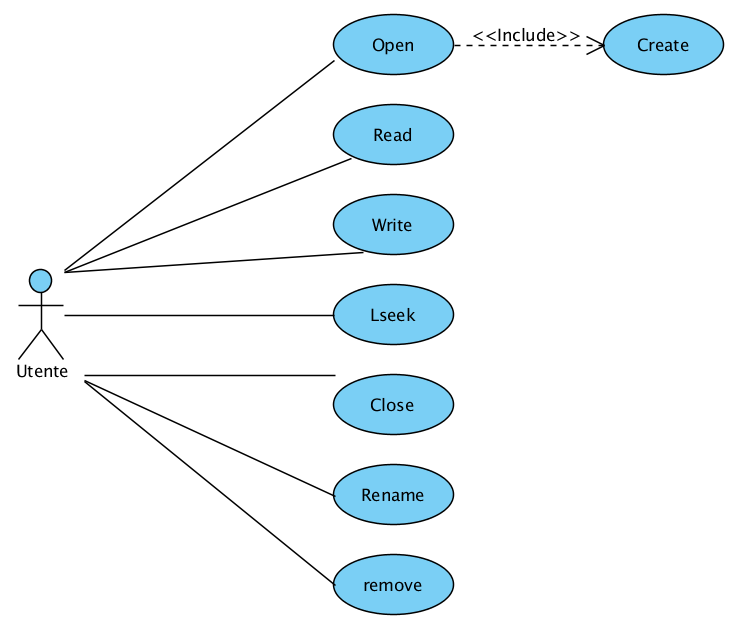
\includegraphics[width=300px,height=200px]{./Immagini/UseCaseFile.png}
	\caption{Diagramma Caso d'uso gestione File}
	\label{Fig.:UseCaseFile}
    \end{figure}

  \newpage

  Elenchiamo le system call per la gestione delle cartelle: \\

    \begin{description}
     \item[mkdir]System call utilizzata per creare una directory.
     \end{description}
     
     \begin{description}
      \item[rmdir]System call che elimina una directory. 
      \end{description}
      
      \begin{description}
       \item[chdir] System call che permette di cambiare la directory corrente. 
       \end{description}

      \begin{description}
     \item[getcwd] System call che riporta la directory corrente. 
    \end{description}

\begin{figure}[h]
 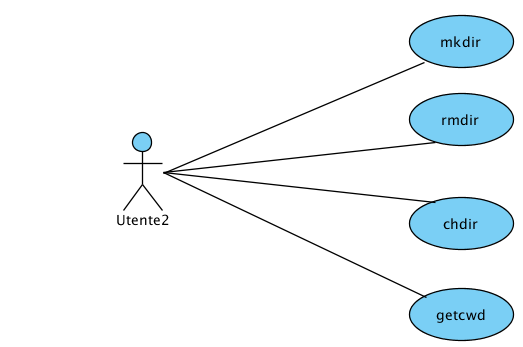
\includegraphics[width=300px,height=150px]{./Immagini/UseDir.png}
\caption{Diagramma Caso d'uso gestione Cartelle}
\end{figure}

\section{Conclusioni}
  In questo capitolo ho presentato i vari obiettivi che il sistema cerca di raggiungere. Nell'analisi dei requisiti software si è fatta un'introduzione molto semplice dell'architettura software, scegliendo di mettere in evidenza il punto di vista dell'utente. Un miglior dettaglio della struttura software è presentato nel capitolo §\ref{cap:Struttutra_Progetto}



\clearpage{\pagestyle{empty}\cleardoublepage}

		\chapter{ Modifiche Introdotte sul nucleo}
\label{cap:Modifiche}
Il file system è un componente complesso del modulo IO, per far fronte a tutte le esigenze di questo componente è stato necessario introdurre alcune modifiche e nuove funzionalità ai moduli di sistema e IO.
Senza l'introduzione di tali modifiche non sarebbe stato possibile realizzare il supporto al file system FAT32, ma nonostante ciò queste non fanno parte del file system.\\	

 \section{Modifiche modulo Sistema}
 Il modulo sistema è il modulo principale del nucleo. Questo modulo viene caricato dal boot loader ed esegue l'inizializzazione delle principali caratteristiche del nucleo quali: la gestione dei processi, la gestione della memoria virtuale, la gestione dei semafori e poi carica i restanti moduli. 
 Le modifiche introdotte su questo modulo riguardano principalmente due aspetti: la gestione dell'hard disk e l'introduzione di una area riservata per ogni processo. 
 \subsection{Hard Disk}
 Il driver dell'hard disk è inserito nel modulo sistema, in quanto necessario per una corretta gestione dell'area di swap. Le modifiche introdotte riguardano la gestione dei volumi di un disco che era assente.Le primitive presenti supportano le operazioni di scrittura e lettura sul disco ma senza aver coscienza del volume sul quale si sta lavorando.\\
 Per un corretto funzionamento del filesystem è stato necessario introdurre delle primitive accessibili solamente a livello sistema che mi hanno permesso di identificare quali volumi sono presenti sul disco ed effettuare operazioni di lettura e scrittura su questi. 
  \begin{description}
   \item[get\_partizione]
   E' una primitiva a livello sistema che permette di accedere alla lista delle partizioni presenti nella memoria del modulo sistema, altrimenti inaccessibile dal modulo IO in quanto  
   non collegati tra di loro. Questa primitiva riporta un indice univoco mediante il quale è possibile riferire la partizione all'interno del disco.
   \end{description}
  \begin{description}
   \item[write\_part\_n]
    Primitiva a livello sistema che permette di eseguire le operazioni di scrittura sulle varie partizioni presenti sul disco.
    Per poter identificare la partizione in modo univoco, associate alle informazioni attinenti il canale ATA e il DRIVER, si deve indicare l'indice
    ottenuto dalla primitiva get\_partizione.
  \end{description}
   \begin{description}
   \item[read\_part\_n]
    Primitiva a livello sistema che permette di eseguire le operazioni lettura sulle varie partizioni presenti sul disco.
    Per poter identificare la partizione in modo univoco, associate alle informazioni attinenti il canale ATA e il DRIVER, si deve indicare l'indice
    ottenuto dalla primitiva get\_partizione.
  \end{description}
  \subsection{Area privata processo}
  \label{AreaPrivataProcesso}
  Il file system per poter gestire correttamente i file e le directory ha la necessità di associare delle informazioni private ad ogni processo. Il nucleo non supportava questa possibilità, quindi è stato necessario introdurre un meccanismo che permettesse di gestire quest'area privata dallo spazio IO.\\
  La prima modifica introdotta riguarda il descrittore di processo nel quale sono stati introdotti dei campi aggiuntivi che permettono di associare e gestire l'area privata di ogni processo.\\
  Le modifiche introdotte sono le seguenti : \\
  
\begin{code}
      natl  p_id; 	    // id del processo padre
      void* iostate;        // puntatore area riservata  
      natl  iostate_size;   // grandezza area riservata 
\end{code}
 

  La prima questione da affrontare, una volta inserite queste modifiche, è come e con quali valori l'area deve essere inizializzata. L'area privata di un processo viene inizializzata durante la creazione del processo copiando i valori contenuti nell'area del processo padre, se questa è presente. \\
  Se l'area del processo padre non è presente, si copiano i valori di default contenuti nell'area di memoria globale inserita nel modulo sistema ed individuata dal puntatore \textit{io\_global\_info}, se è stata inizializzata. Se non è presente nessun area globale, l'area privata del processo non viene inizializzata.\newpage
  Per supportare la procedura sopraccitata ho modificato la crea\_processo nel seguente modo. \\
  
 \begin{code}
	pdes_proc->p_id = esecuzione->id;
 	father_proc=des_p(esecuzione->id); 
	
	// non puo esistere la condizione nella
	// quale le informazioni globali non sono  
	// inizzializatementre quelle del padre si,
	// il contrario invece puo capitare
	// ( processo main ) 

 	if(io_global_info && io_global_size 
	      && father_proc->iostate &&
	      father_proc->iostate_size ) { 
 	    // copio le informazioni del padre 
  	    natl size=father_proc->iostate_size; 
  	    pdes_proc->iostate_size=size; 
  	    pdes_proc->iostate=alloca(size, 1); 
  	    if (!pdes_proc->iostate) goto errore6; 
  	    memset(pdes_proc->iostate, 0, size); 
  	    memcpy(pdes_proc->iostate,father_proc->iostate,size); 
   
 	}else if (io_global_info && io_global_size) { 
	   // se il padre non ha informazioni copio quelle globali 
	    pdes_proc->iostate_size=io_global_size; 
 	    pdes_proc->iostate=alloca(io_global_size, 1); 
 	    if (!pdes_proc->iostate) goto errore6; 
 	    memset(pdes_proc->iostate, 0, io_global_size); 
 	    memcpy( pdes_proc->iostate,io_global_info,io_global_size); 
	   
	} else {
	  //azzero le informazioni riguardanti l'area IO
	    pdes_proc->iostate=NULL; 
	    pdes_proc->iostate_size=0; 
	}
   }
  
\end{code}


  Questa area però deve anche essere dealocata, questo compito viene eseguito all'interno della \textit{distruggi\_processo}.\\
  Poiché l'area privata è stata inserita nello spazio di indirizzamento di sistema, per il file system e qualunque altro componente del modulo IO è impossibile accedere alle informazioni presenti nei descrittori di processo, e di conseguenza all'area privata.\\ 
  Per gestire quest'area in modo corretto ho inserito le seguenti primitive accessibili solo da livello sistema : 
  \begin{description}
   \item[c\_io\_space\_init]
    Primitiva che inizializza l'area globale presente nel modulo sistema. Questa primitiva alloca lo spazio necessario per inserire i valori ricevuti come parametri. 
  \end{description}
  \begin{description}
   \item[c\_io\_space\_read]
   Primitiva che consente di leggere dei valori nell'area privata di un processo, specificando un offset di interesse.
  \end{description}
    \begin{description}
   \item[c\_io\_space\_write]
   Primitiva che consente di scrivere dei valori nell'area privata di un processo, specificando un offset di interesse.
  \end{description}

  
 \section{Modifiche modulo IO}
 Nel modulo IO è inserito il file system che verrà discusso ampiamente nei prossimi capitoli, in questo paragrafo mi limito a mostrare le modifiche introdotte nel modulo IO non facenti parte del file system. \\
 Nel modulo IO le principali modifiche che ho introdotte sono: l'introduzione di un sistema per la gestione dell'ora e della data, l'introduzione di una semplice gestore degli errori e l'introduzione di  alcune librerie.
 \subsection{Data e ora}
 Il nucleo non possiede nessun meccanismo per ottenere ne l'ora corrente, ne la data corrente. Ogni computer è munito di un sistema per mantenere la data e l'ora dopo lo spegnimento del computer, questo sistema e formato da una memoria CMOS e da un RTC accessibili mediante delle porte di IO.\\
 Per usare questo dispositivo ho realizzato un piccolo driver gestito a controllo di programma che mi permette di leggere la data e l'ora contenute nei suoi registri e operare le opportune conversioni sui valori letti fornendomi un'interfaccia semplice ed omogenea.\\
 Per usufruire di questo meccanismo ho inserito due primitive accessibili anche da livello utente : 
 \begin{description}
  \item[get\_time]
    Primitiva di livello utente che riporta l'ora corrente. L'ora corrente viene restituita in un formato compatto, di grandezza pari a 4 byte, ogni byte assume un significato particolare. 
    \begin{itemize}
     \item Byte 0: Contiene il valore del secondo corrente espresso in formato binario. Range [0-59]. 
    \end{itemize}
    \begin{itemize}
     \item Byte 1: Contiene il valore del minuto espresso in formato binario. Range [0-59].  
    \end{itemize}
    \begin{itemize}
     \item Byte 2: Contiene il valore dell'ora corrente espresso in formato binario.Range [0-23].
    \end{itemize}
    \begin{itemize}
     \item Byte 3: Byte inutilizzato a disposizione.
    \end{itemize}
  \end{description}
  
  \ \begin{description}
  \item[get\_data]
    Primitiva di livello utente che riporta la data corrente. La data corrente viene restituita in un formato compatto, di grandezza pari a 4 byte, ogni byte assume un significato particolare. 
    \begin{itemize}
     \item Byte 0: Contiene il valore del giorno corrente espresso in formato binario. Range [1-31].   
    \end{itemize}
    \begin{itemize}
     \item Byte 1: Contiene il valore del mese corrente  espresso in formato binario. Range [1-12].
    \end{itemize}
    \begin{itemize}
     \item Byte 2: Contiene il valore dell'anno corrente espresso in formato binario. Range [0-99].
    \end{itemize}
    \begin{itemize}
     \item Byte 3: Byte inutilizzato a disposizione.
    \end{itemize}
  \end{description}
 
\subsection {Librerie}
 \label{lib}
  Data l'ampiezza del progetto è stato necessario implementare delle librerie più meno standard che utilizzo in quasi tutti i moduli. 
  Le librerie introdotte vengono linkate al modulo IO, quindi sono disponibili per tutto il sistema IO.
  
  \begin{description}
    \item[string.h]
    Libreria standard C, dove sono presenti le principali funzioni per la gestione delle stringhe.
  \end{description}
  
  
  \begin{description}
    \item[strarg.h]
    Libreria standard C, sono presenti le macro e le funzioni per la gestione degli argomenti delle funzioni.
  \end{description}
  
  
  \begin{description}
    \item[wchar.h]
    Libreria standard C, dove sono presenti le principali funzioni per la gestione delle stringhe in formato wchar.
  \end{description}
  
  \begin{description}
    \item[error.h]
    Libreria standard C, piccola libreria che permette di gestire in modo molto semplice gli errori a livello sistema.
  \end{description}
  
 \subsection{Gestione errori}
    Sempre a causa dell' ampiezza del progetto, è stato necessario introdurre una semplice gestione degli errori. L'implementazione di questo 
    avviene nella libreria errno.h. \\
    Questa gestione viene realizzata principalmente mediante delle funzioni che agiscono su delle variabili globali che contengono lo stato attuale.  
     \begin{itemize}
      \item \textbf{errno} : word che contiene un codice identificativo per l'errore che si è verificato. 
     \end{itemize}
     
    \begin{itemize}
     \item \textbf{str\_errno} : stringa che contiene la spiegazione dell'errore contenuto in errno. 
    \end{itemize}

    Nonostante sia possibile accedere direttamente alle variabili e modificarne il contenuto, è consigliato usare le successive funzioni messe a disposizione dalla libreria errno.h. 
    
      \begin{description}
       \item[perror]
	    Funzione che stampa la stringa di errore accodata alla stringa passata come argomento
       \end{description}

  \begin{description}
   \item[set\_errno] 
	    Funzione che setta le variabili di errore globali ai valori specificati come argomento.
   \end{description}
    
   \begin{description}
    \item[reset\_errno]
	Funzione che resetta le variabili di errore, inserendo il valore di default (successo).  
   \end{description}

    \section{Conclusioni}
      In questo capitolo sono state presentate in maniera generica tutte le modifiche riguardanti il nucleo. \\
      Per maggiori informazioni si rimanda ai sorgenti, che sono accompagnati da una discreta quantità di commenti. \\
\clearpage{\pagestyle{empty}\cleardoublepage}
		\chapter{Struttura del progetto}
\label{cap:Struttutra_Progetto}
In questo capitolo mostro l'architettura software del progetto, mettendo in
evidenza i moduli di cui è composto e le varie relazioni che sussistono tra di loro.\\
Prima di tutto bisogna definire il concetto di modulo :     
       \begin{quote}
       \textit{``Un \textbf{modulo software} è una porzione di software, che
	contiene e fornisce servizi o risorse e a sua volta può usufruire di risorse o
	servizi offerti da altri moduli.\\ L'insieme dei servizi 
	messi a disposizione prende il nome di \textit{interfaccia}.''}
       \end{quote}

Si è deciso di adottare una struttura modulare per ottenere una maggior
chiarezza e una più semplice gestione del sistema file system. 
Ogni modulo è composto da una o più componenti, ognuna delle quali svolge un compito
ben preciso. \\ 
Il principale vantaggio di questo approccio è quello che,  qualora si volessero
introdurre delle modifiche, per ottenere miglioramenti o nuove funzionalità, queste riguarderebbero solo 
il modulo interessato senza che ciò comporti variazioni o malfunzionamenti sugli altri moduli.\\
Per esempio se uno volesse introdurre una cache delle scritture, questa modifica
riguarderebbe solamente il modulo a cui è stato assegnato il compito di gestire
la zona dati del disco, mentre gli altri moduli non 
subirebbero modifiche. 

\section{Struttura Modulare}
\label{sech:Struttura_Modulare}
Il File system è composto da tre macro-moduli, che riprendono la struttura
generale di un file sytem vista nel precedente capitolo §\ref{cap:FileSystem}. Seguendo un
approccio bottom-up descriviamo il funzionamento generale di questi moduli.
\begin{description}
 \item[Modulo Base]
    Il primo modulo è il modulo base. Lo scopo di questo modulo è di
interfacciarsi con il driver del disco e di fornire al modulo superiore un
interfaccia con la quale gestire le regioni FAT e Data del disco. 
 \end{description}
\begin{description}
 \item[Modulo Gestore File]
  Il secondo Modulo è il modulo intermedio, che esegue la gestione logica dei file.
  Si occupa della gestione entry FAT e dei nomi. Fornendo un'interfaccia
  semplice al modulo superiore mediante la quale si possono gestire i file tramite il concetto di file control block ( spiegato nel paragrafo §\ref{sez:Req} ).
 \end{description}
\begin{description}
 \item[Modulo File system logico]
 Mette a disposizione le system call usate dall'utente finale, e traduce le informazioni ottenute dall'utente in informazioni comprensibili ai livelli inferiori. 
 \end{description}
Sia le comunicazioni tra i vari moduli del sistema, sia le comunicazioni tra i moduli e i componenti esterni appartenenti al nucleo avvengono mediante opportune strutture dati.  
Ogni modulo conosce la struttura dati del modulo precedente e di quella del modulo successivo. \\
La figura \ref{Fig:StrutturaFS} riassume con semplicità questo concetto. 
Le strutture dati sono individuate dal nome posto sopra i link che collegano i vari moduli. Nei paragrafi successivi, le strutture dati verrano analizzate con un miglior detaglio.\\

\begin{center}
\begin{figure}[h]
 \centering
 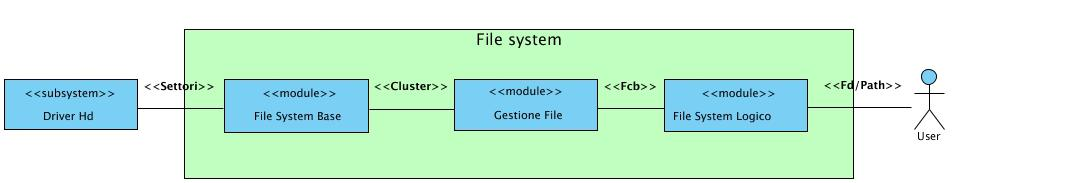
\includegraphics[width=400px,height=70px]{./Immagini/FS.jpg}
 % FS.jpg: 1070x183 pixel, 96dpi, 28.31x4.84 cm, bb=0 0 803 137
 \caption{Struttura generale del sistema.}
 \label{Fig:StrutturaFS}
\end{figure}\end{center}

\section{Modulo Base}
\label{sect:ModuloBase}
Il modulo base è il modulo che si occupa della gestione a basso livello del file system. Lo scopo è quello di gestire in modo corretto le zone dati e FAT del disco e di mostrare ai livelli superiori un'
interfaccia semplice con la quale interagire. 
Il compito di questo modulo rimane comunque molto complesso, si è perciò deciso di scomporlo in componeti più semplici a ciascuno dei quali è stato assegnato uno scopo specifico.\\
Di seguito verrano illustrati i singoli componenti. 
 
\subsection{Volume}
  Il primo componente chiamato dal sistema è il componente Volume. Questo ha il compito di analizzare il disco alla ricerca delle partizioni FAT. Una volta individuata crea la relativa struttura e la  inserisce nella tabella dei volumi. \\
  La \textit{tabella dei volumi} è una struttura globale, necessaria ai moduli superiori per una corretta gestione dei volumi presenti nei dischi. E' una struttura molto semplice realizzata mediante una lista concatenata nella quale vengono inseriti tutti i moduli rilevati. \\
  Per ogni volume sono presenti due semafori di mutua esclusione, uno riservato alla gestione della Regione Dati e l'altro per la Regione FAT.
  Sono inoltre presenti informazioni riguardanti la formattazione del volume, un puntatore alla FAT in memoria e un puntatore al FCB della root.\\

  Il modulo mette a disposizione la seguente interfaccia : \\	
    \begin{description}
     \item[crea\_tabella\_volumi]
    Questa funzione ha lo scopo di creare la tabella dei volumi.  La funzione per poter creare la tabella cerca nel disco mediante la primitiva di sistema get\_partizione le partizioni fat, una volta identificate crea  ed inserisce nella lista un nuovo elemento. Nell'elemento inserirà tute le informazioni attinenti a quel volume, assegnerà un etichetta univoca e creerà ed inizializzerà il FCB della root directory. \\
    \end{description}
    
    \begin{description}
     \item[print\_tabella]
	E' una funzione di debug, che viene usata per stampare a video il contenuto della tabella. \\
     \end{description}
     
    \begin{description}
     \item[get\_volume]
	 E' una funzione di utilità necessaria per rintracciare un determinato volume mediante l'etichetta. \\
     \end{description}
 
    \begin{description}
      \item[delete\_tabella]
	E' Funzione che viene chiamata esclusivamente in caso di errore per rilasciare le varie zone dati allocate.\\
     \end{description}

\section{Fat}	
  Il Secondo componente del modulo base è il componente FAT. Questo ha il compito di gestire in modo corretto la tabella FAT. A questo livello tutti i file vengono gestiti mediante le catene di cluster che sono salvate
  nella FAT. Quindi, il compito principale di questo componente è quello di offrire un'interfaccia semplice che permetta la creazione, la modifica e l'eliminazione di queste catene.\\
  Per questioni di efficienza si è scelto di caricare la tabella FAT in memoria, ciò comporta però un inconveniente, infatti la tebella FAT in memoria deve essere sempre in uno stato consistente con quella presente nel disco. Tutte le scritture devono comportare una scrittura sia nel disco e sia nella memoria e poiché si potrebbero verificare delle inconsistenze tra i dati le scritture devono avvenire in mutua esclusione tra loro. 
  Questa procedura è regolata dal semaforo presente nel volume associato alla tabella FAT corrispondente.\\

  Il modulo esporta la seguente interfaccia  : \\
   
  \begin{description}
   \item[delete\_memory\_fat] Funzione che elimina la tabella FAT dalla memoria solitamente usata in casi di errore.
  \end{description}
    \begin{description}
   \item[get\_next\_fat]Funzione utilizzata per scorrere una catena FAT. Questa funzione esegue dei controlli sulla consistenza della catena stessa.
  \end{description} 
    \begin{description}
   \item[init\_fat]Funzione che carica in memoria la tabella FAT.  
   \end{description}
  \begin{description}
   \item[create\_fat ] Funzione che crea una nuova catena FAT.
  \end{description}  
  \begin{description}
   \item[append\_fat]Funzione che aggiunge un cluster alla catena.
  \end{description}
  \begin{description}
   \item[delete\_fat]Funzione che elimina l'ultimo cluster dalla catena.
  \end{description}   
  \begin{description}
   \item[delete\_fat\_all]Funzione che elimina tutta la catena.
  \end{description}     
 \begin{description}
  \item[print\_chain] Funzione di debug che stampa a video la catena. 
  \end{description}     
    

\subsection{DATA}
\label{sec:Data}
  L'ultimo componente presente nel modulo base è il componente data, che ha lo scopo di gestire la zona dati. \\
  Questo componente mette a disposizione degli altri moduli le funzioni di scrittura e lettura sul disco.\\
  I moduli che usano queste funzioni devono fornire solamente la catena di cluster sulla quale si vuole scrivere e l'offset di scrittura, in questo modo si offre un visione
  uniforme dello spazio del disco, semplificando le operazioni di lettura e scrittura per i moduli superiori.\\
  
  Il modulo esporta la seguente interfaccia: 
    \begin{description}
     \item[write\_data] Funzione che scrive  sulla catena di cluster specificata come argomento, all'offset specificato.
     \end{description}
    \begin{description}
     \item[read\_data]  Funzione che legge sulla catena di cluster specificata come argomento, all'offset specificato.
    \end{description}
  Queste sono le uniche due funzioni che vengono usate per l'accesso ai dati nel disco. 

  \begin{figure}[!h]
 \centering
  \textheight 10px
 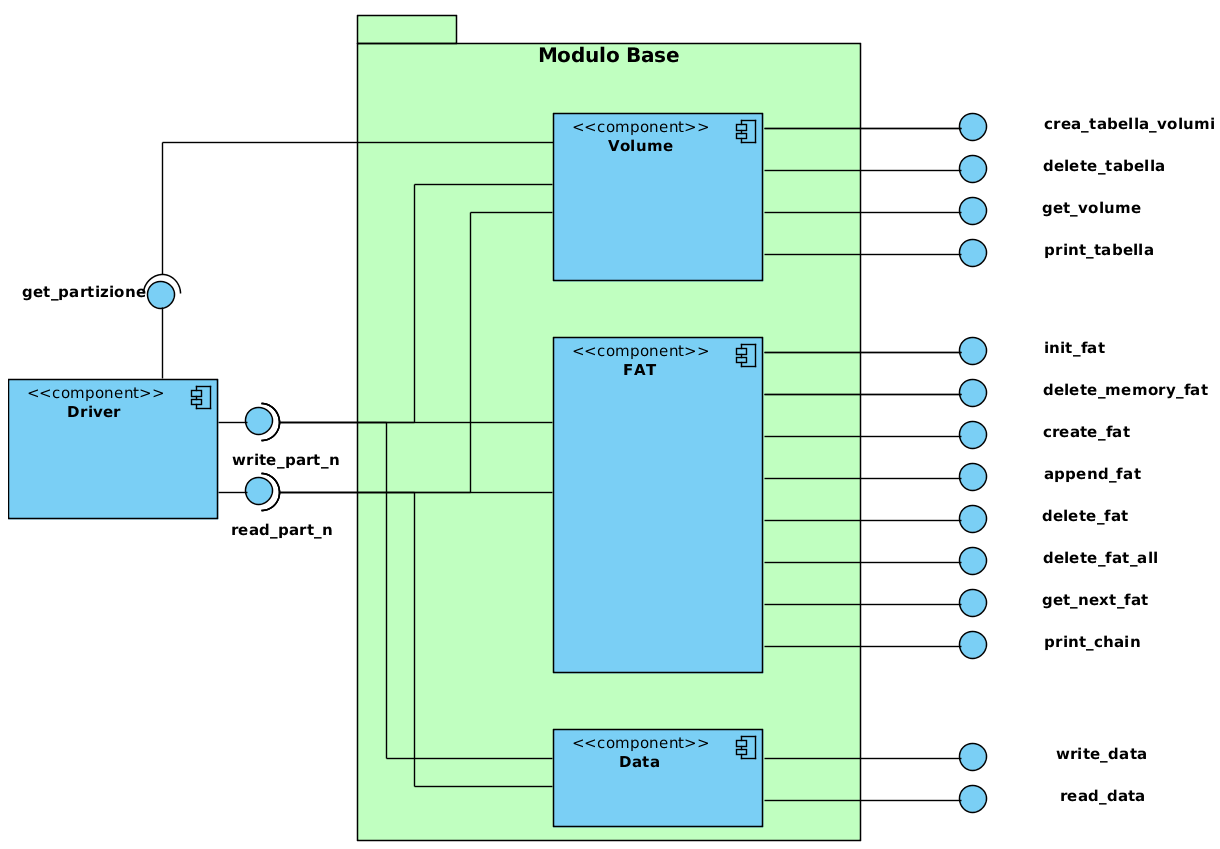
\includegraphics[width=400px,height=300px]{./Immagini/Base.png}
 % Base.png: 1220x849 pixel, 96dpi, 32.28x22.46 cm, bb=0 0 915 637
 \caption{Modulo Base}
 \label{fig:Base}
\end{figure}

\newpage 

\section{Modulo Gestore dei File}
 Il modulo Gestore dei file è il modulo che fa da intermediario tra il modulo base e quello logico.
  La funzionalità principale di questo modulo è quella di gestire i file e le cartelle. 
 Il modulo intermedio colloquia con il modulo logico mediante una struttura dati che prende il nome di \textbf{file control block (FCB)}. 
 Questa struttura è di fondamentale importanza per la gestione dei file, la tabella successiva ne riassume i vari campi.
  
\begin{center}
\begin{tabular}{|l|l|}\hline
\textbf{Campo} & \textbf{Significato}\\\hline
volume & Puntatore al volume nel quale è presente il file\\\hline
cluster & Numero del primo cluster\\\hline
type & Flag presente nella short entry\\\hline
mode & Modalita di apertura\\\hline
pos\_corr & Posizione corrente nel file\\\hline
size & Grandezza del file\\\hline
cluster\_father & Cluster della direcotory nel quale inserito\\\hline
offset\_father & Offset all'interno della directory\\\hline
n\_entry & Numero entry di cui è composto\\\hline
\end{tabular}
\end{center}

È la struttura nella quale sono presenti tutte le informazioni necessarie per la gestione dei file. \\

  \subsection{Direntry}
    Il componente direntry, è il componente principale di questo modulo. Lo scopo di questo componente è quello di gestire le strutture dati che contengono le informazioni dei file. 
    Nella gestione delle entry dei file si sono seguite le specifiche Microsoft in modo pedissequo. \\
    Il sistema è in grado di rilevare e gestire in maniera corretta file formati da entry lunghe più entry corte, file formati da sole entry corte (vedi \ref{gest:dir}). \\
    Si è prestato particolare cura nella realizzazione dell'algoritmo per la generazione dei nomi corti. In particolare nel caso di nomi simili\footnote{Per il concetto di Nomi simili si intendono nomi uguali per i primi 8 caratteri.},
   l'algoritmo genera il numero corretto, controllando che nel disco non sia già presente un file con quel nome. Nel caso si arrivi alla presenza di 10 file con i nomi simili nella stessa cartella, il sistema 
   genererà il nome corto in modo casuale. \\
  L'interfaccia esportata da questo modulo è la seguente : 

    \begin{description}
     \item[open\_entry]
     Funzione che effettua la ricerca di un file e se presente inizializza il FCB associato. 
     \end{description}

    \begin{description}
     \item[delete\_entry]
      Funzione che elimina un entry. Se presente una catena di cluster associata all'entry oggetto dell'eliminazione, anche questa verrà rimossa. 
     \end{description}
   
    \begin{description}
      \item[create\_entry]
      Funzione che crea un entry ed inizializza il FCB associato. 
    \end{description}

    \begin{description}
     \item[rename\_entry]
      Funzione che modifica il nome di un entry. Modifica opportunamente il FCB associato.   
   \end{description}

    \begin{description}
     \item[create\_directory]
      Funzione che crea una directory vuota. Inizializza in modo opportuno il FCB associato. 
     \end{description}

    \begin{description}
     \item[delete\_directory]
      Funzione che elimina una directory vuota. 
     \end{description}
  

  \subsection{FCB}
    Questo componente è molto semplice, contiene la definizione della struttura dati FCB vista precedentemente. Inoltre in questo componente ho inserito le funzioni che permettono la scrittura e la lettura
    usando i FCB per individuare  il file o la directory.  Il loro compito e solo quello di estrarre le informazioni dal FCB , chiamare le funzioni read\_data e write\_data presenti nel modulo inferiore e 
    aggiornare se necessario i campi del FCB. 
  
  \newpage

  \begin{figure}[h]
 \centering
 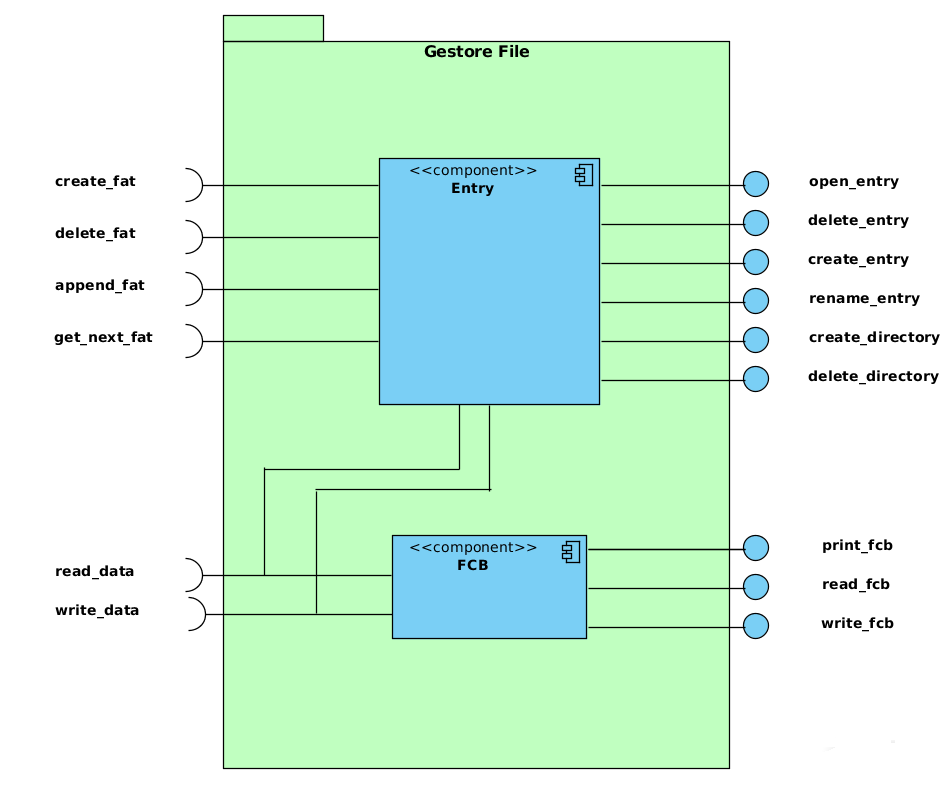
\includegraphics[width=400px,height=350px]{./Immagini/GestoreFile.png}
 % GestoreFile.png: 949x788 pixel, 96dpi, 25.11x20.85 cm, bb=0 0 712 591
 \caption{Gestore File}
 \label{fig:GestoreFile}
\end{figure}


\section{System Call}
\label{sec:Logico} 
   Il modulo system call è il modulo che implementa tutte le system call esportate a livello utente. \\		
   Il compito principale di questo modulo è quello di elaborare le informazioni ottenute dall'utente ed inizializzare gli opportuni Fcb con i quali chiamare le funzioni del livello precedente. 
   Un ulteriore compito di questo è quello di gestire le aree di memoria riservate nel modulo sistema necessarie per il salvataggio delle informazioni private per ogni processo, mediante le primitive viste nel paragrafo § \ref{AreaPrivataProcesso}.\newpage
   L'interfaccia esportata da questo modulo coincide con le system call appartenenti al file system : \\
          
     
     \begin{description}
      \item[open]
	System call che apre il file specificato dall'utente. Si occupa di creare il relativo FCB ed inserirlo nell'area privata del processo.
	Riporta il file descriptor associato al file oggetto della chiamata.\\
	Il file può essere aperto nelle seguenti modalità : \\
	  \begin{itemize}
	   \item O\_RDONLY   :   apre il file in sola lettura.\\			
 	   \item O\_WRONLY   :   apre il file in sola scrittura.\\				
 	   \item O\_RDWR     :   apre il file in lettura/scrittura.\\			
 	  \item  O\_CREAT    :   se il file non esiste verrà creato.\\			
 	   \item O\_DIRECTORY :   se il path specificato non è una directory la chiamata fallisce  \\ 
       \end{itemize}
     \end{description}
      
      \begin{description}
       \item[close]
	System call che chiude il file specificato dall'utente mediante il file descriptor. Inoltre rimuove il Fcb associato al file oggetto della chiamata.
       \end{description}
       
       \begin{description}
        \item[read] System call usata per leggere i dati da un file. Il file deve essere stato precedentemente aperto.
       \end{description}

        \begin{description}
         \item[write] System call usata per scrivere i dati su un file. Il file deve essere stato precedente aperto. 
         \end{description}

     \begin{description}
      \item[lseek] System call usata per spostare la posizione corrente su un file.Il file deve essere stato precedentemente aperto. 
      Si può inoltre indicare il punto di partenza dal quale inserire l'offset usando i seguenti parametri : \\
	\begin{itemize}
	 \item SEEK\_SET si fa riferimento all'inizio del file,  
	      il valore (sempre positivo) di offset indica direttamente la nuova posizione corrente.        
	 \item SEEK\_CUR si fa riferimento alla posizione corrente del file,  ad essa viene sommato offset (che può essere negativo 
	      e positivo) per ottenere la nuova posizione corrente. 
	\item  SEEK\_END si fa riferimento alla fine del file, alle dimensioni  del file viene sommato offset (che può essere negativo  e positivo) per ottenere la nuova posizione corrente.  
	\end{itemize}

      \end{description}
    
    \begin{description}
     \item[remove] System Call il cui scopo è rimuove un file. Il file non deve essere stato aperto in precedenza. 
     \end{description}
     
     \begin{description}
      \item[rename] System Call il cui scopo è rinominare un file.Il file non deve essere stato aperto in precedenza. 
      \end{description}

    \begin{description}
     \item[mkdir]System call il cui scopo è di creare una directory.
     \end{description}
     
     \begin{description}
      \item[rmdir] System call il cui scopo è di eliminare una directory, solamente se questa è vuota. 
      \end{description}
      
      \begin{description}
       \item[chdir] System call il cui scopo è di modificare la directory corrente associata al processo. 
       \end{description}

      \begin{description}
     \item[getcwd] System call il cui scopo è di riportare la directory corrente associata la processo. 
    \end{description}
  
\begin{figure}[h]
 \centering
 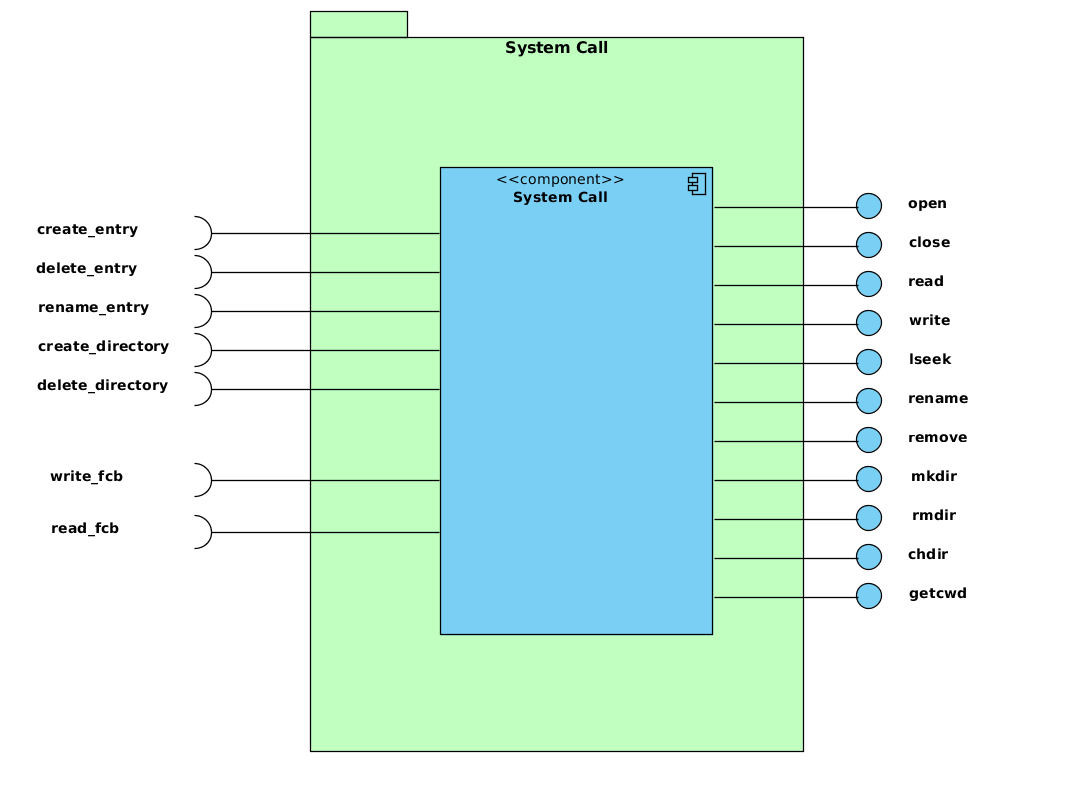
\includegraphics[width=350px,height=280px]{./Immagini/system_call.png}
 % system_call.png: 1084x788 pixel, 96dpi, 28.68x20.85 cm, bb=0 0 813 591
 \caption{ Modulo SystemCall}
 \label{fig:SystemCall}
\end{figure}


\section {Processo di Inizializzazione}
   Il processo di inizializzazione non è un modulo come quelli presentati precedentemente. Ho scelto di inserirlo in questa sezione poiché ricorrerò ai concetti presentati nei paragrafi precedenti. 
  
   E' rappresentato dalla funzione \textbf{fs\_init}, che ha il compito di inizializzare il file system. 
   Questa funzione invoca le funzioni di inizializzazione dei moduli. La prima azione che viene eseguita è la creazione della tabella dei volumi, successivamente vengono caricate in memoria le tabelle FAT dei vari volumi ed infine viene inizializzata l'area privata del processo di IO. L'inizializzazione dell'area privata del processo di IO, fa sì che tutti i suoi processi figli ereditino le informazioni dal padre.\\ 
  
\section {Conclusioni}
  In questo capitolo abbiamo presentato la struttura generale del sistema, mettendo in evidenza i vari moduli, componenti e interfacce mediante le quali colloquiano.
  Non ci siamo addentrati nei dettagli implementativi, per questi si rimanda ai sorgenti del sistema, che sono accompagnati da una discreta quantità di commenti per agevolarne la comprensione. 
  
\clearpage{\pagestyle{empty}\cleardoublepage
		%\lstinputlisting{fat.c}
		%\input{stato_arte.tex}
		%\input{progetto.tex}
%	\backmatter
	%	\appendix
	%		\input{appendiceA.tex}
		%\appendix
		%	\input{appendiceB.tex}
		\begin{thebibliography}{100}
\bibitem{Sistemi Operativi} \emph {Sistemi Operativi Concetti ed esempi} \\ A.Silberschartz-P.B Galvin -G. Gagne 
\bibitem{Architettura dei Calcolatori Volume I} \emph{Architettura dei Calcolatori Volume I} \\ Graziano Frosini Giuseppe Lettieri
\bibitem{Architettura dei Calcolatori Volume I} \emph{Architettura dei Calcolatori Volume II} \\ Graziano Frosini Giuseppe Lettieri
\bibitem{Architettura dei Calcolatori Volume I} \emph{Architettura dei Calcolatori Volume III} \\ Graziano Frosini Giuseppe Lettieri
\bibitem{Fat} Microsoft \emph{FAT specifiche generiche} \\ \url {http://msdn.microsoft.com/it-it/windows/hardware/gg463084}
\bibitem{Long Name} Microsoft \emph{Specifiche gestione nomi FAT32} \\ \url {www.osdever.net/documents/LongFileName.pdf}
\bibitem{FatDev} Os-dev Fat \\ \url {http://wiki.osdev.org/FAT}
\bibitem{CMOS} Os-dev CMOS \\ \url {http://wiki.osdev.org/CMOS}
\bibitem{RTC} Os-dev RTC \\ \url {http://wiki.osdev.org/RTC}
\end{thebibliography}
\clearpage{\pagestyle{empty}\cleardoublepage}

		\appendix
%\chapter{glossario} 
%\begin{multicols}{2} 
%\begin{description} 
%\item[voce 1] spiegazione 
%\item[voce 2] spiegazione 
%\end{description} 
%\end{multicols}
\end{document}
